% Copyright (C) 2010-2018 The ESPResSo project
% Copyright (C) 2002,2003,2004,2005,2006,2007,2008,2009,2010 
%   Max-Planck-Institute for Polymer Research, Theory Group
%  
% This file is part of ESPResSo.
%   
% ESPResSo is free software: you can redistribute it and/or modify it
% under the terms of the GNU General Public License as published by the
% Free Software Foundation, either version 3 of the License, or (at your
% option) any later version.
%  
% ESPResSo is distributed in the hope that it will be useful, but
% WITHOUT ANY WARRANTY; without even the implied warranty of
% MERCHANTABILITY or FITNESS FOR A PARTICULAR PURPOSE.  See the GNU
% General Public License for more details.
%  
% You should have received a copy of the GNU General Public License
% along with this program.  If not, see <http://www.gnu.org/licenses/>.
%


\documentclass[
a4paper,                        % paper size
11pt,                           % font size
twoside,                        % two sided
footsepline,                    % add a line to separate the footer
headsepline,                    % add a line to separate the header
headexclude,                    % header does not belong to the text
footexclude,                    % footer does not belong to the text
pagesize,                       % set the pagesize in a DVI document
]{scrartcl}

\usepackage[version=4]{mhchem}
\usepackage{hyperref}
\usepackage{graphicx}
\usepackage{fancyvrb}

% Copyright (C) 2010-2019 The ESPResSo project
% Copyright (C) 2002,2003,2004,2005,2006,2007,2008,2009,2010
%  Max-Planck-Institute for Polymer Research, Theory Group
%  
% This file is part of ESPResSo.
%   
% ESPResSo is free software: you can redistribute it and/or modify it
% under the terms of the GNU General Public License as published by the
% Free Software Foundation, either version 3 of the License, or (at your
% option) any later version.
%  
% ESPResSo is distributed in the hope that it will be useful, but
% WITHOUT ANY WARRANTY; without even the implied warranty of
% MERCHANTABILITY or FITNESS FOR A PARTICULAR PURPOSE.  See the GNU
% General Public License for more details.
%  
% You should have received a copy of the GNU General Public License
% along with this program.  If not, see <http://www.gnu.org/licenses/>.
%
\usepackage[draft]{varioref}    % defines \vref
\usepackage{hyperref}           % automatically creates links when
                                % using pdflatex, defines \url
\usepackage{ifpdf}              % defines \ifpdf
\usepackage{graphicx}           % handles graphics
\usepackage{color}              % use colors

\usepackage{amsmath}

\usepackage{verbatim}           % required for \verbatim and \endverbatim
\usepackage{fancyvrb}
\usepackage{calc}               % compute length
\usepackage{ifthen}             % provide ifthen
\usepackage{xspace}
\usepackage{units}
\usepackage[numbers]{natbib}

\usepackage{listings}

% For building the distribution docs, disable todo boxes.
%\usepackage[disable]{todonotes}
\usepackage{todonotes}

\newcommand{\es}{\mbox{\textsf{ESPResSo}}\xspace}
\newcommand{\ie}{\textit{i.e.}\xspace}
\newcommand{\eg}{\textit{e.g.}\xspace}
\newcommand{\etal}{\textit{et al.}\xspace}

\newcommand{\codebox}[1]%
{\texttt{#1}}

\DefineVerbatimEnvironment{code}{Verbatim}%
{commandchars=\\\{\}}
\makeatletter
\newenvironment{tclcode}
{%
  \addtolength{\linewidth}{-2em}% set the line length
  \@minipagetrue%%%DPC%%%
  \@tempswatrue%%%DPC%%%
  \hsize=\linewidth%
  \setbox0=\vbox\bgroup\verbatim
}{\endverbatim
  \unskip\setbox0=\lastbox%%%DPC%%%
  \egroup
  \par%
  \noindent\hspace{1em}%
  \codebox{\box0}%
  \par\noindent%
}
\makeatother

% \newcommand{\todo}[1]{
%   \marginpar{%
%     \setlength{\fboxrule}{1pt}
%     \fcolorbox{red}{yellow}{%
%       \parbox{\marginparwidth-2\fboxrule-2\fboxsep}{%
%         \bf\raggedright\scriptsize #1%
%       }%
%     }%
%   }%
% }

\makeatletter
\renewcommand{\minisec}[1]{\@afterindentfalse \vskip 1.5ex
  {\parindent \z@
    \raggedsection\normalfont\sffamily\itshape\nobreak#1\par\nobreak}%
  \@afterheading}
\makeatother

\newcommand{\esptitlehead}{
  \titlehead{
    \begin{center}
      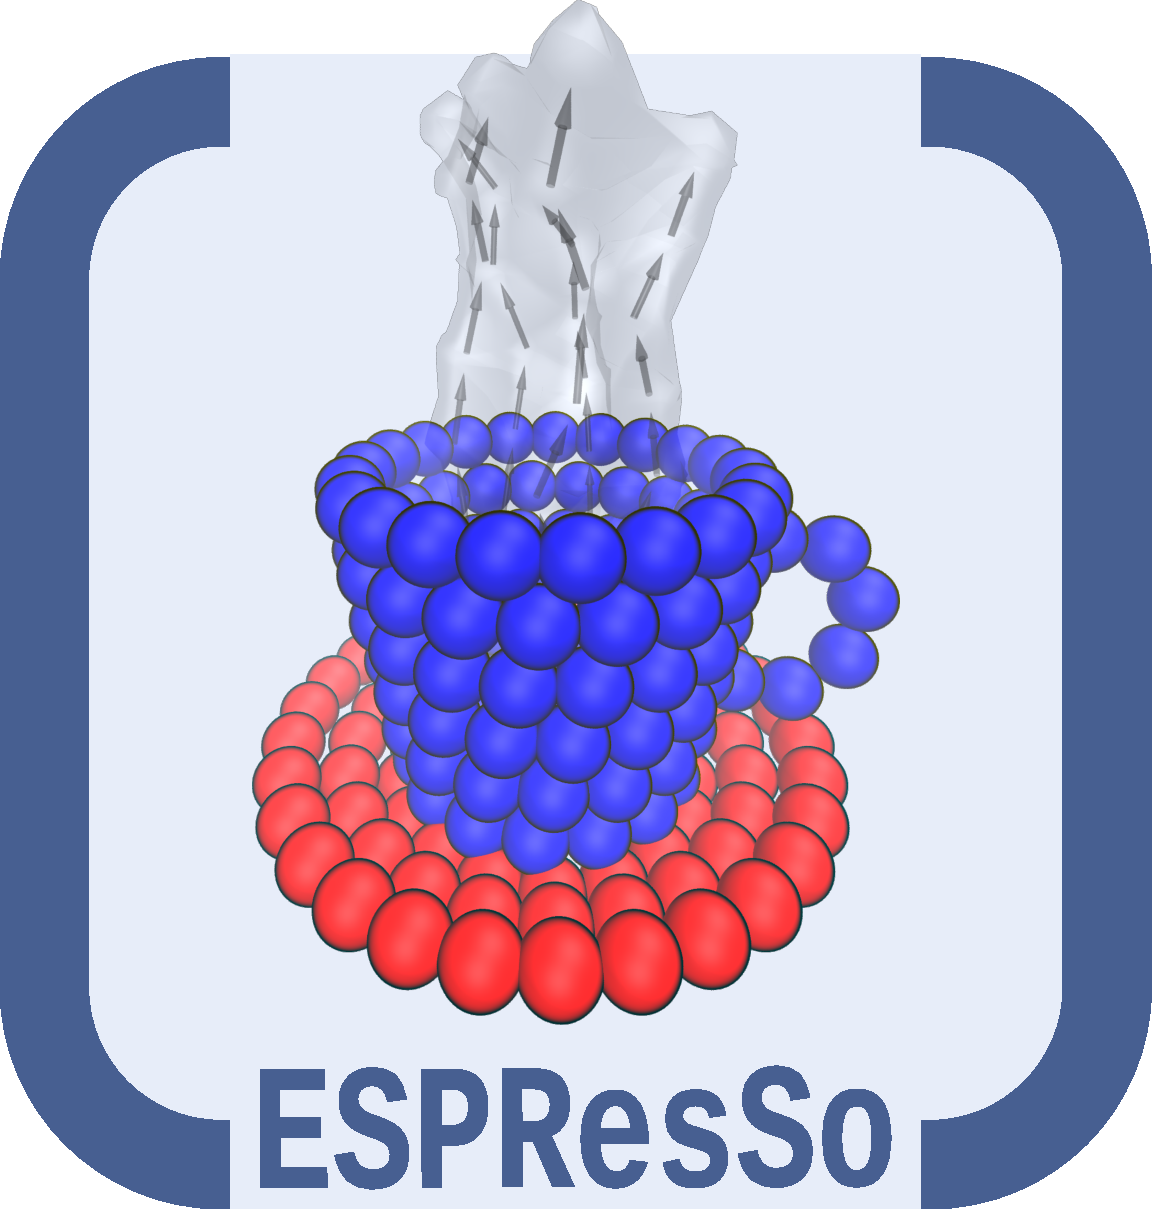
\includegraphics[width=5cm]{logo/logo.pdf}
    \end{center}
  }
}

% Copyright (C) 2010-2019 The ESPResSo project
% Copyright (C) 2002,2003,2004,2005,2006,2007,2008,2009,2010
%  Max-Planck-Institute for Polymer Research, Theory Group
%  
% This file is part of ESPResSo.
%   
% ESPResSo is free software: you can redistribute it and/or modify it
% under the terms of the GNU General Public License as published by the
% Free Software Foundation, either version 3 of the License, or (at your
% option) any later version.
%  
% ESPResSo is distributed in the hope that it will be useful, but
% WITHOUT ANY WARRANTY; without even the implied warranty of
% MERCHANTABILITY or FITNESS FOR A PARTICULAR PURPOSE.  See the GNU
% General Public License for more details.
%  
% You should have received a copy of the GNU General Public License
% along with this program.  If not, see <http://www.gnu.org/licenses/>.
%
\usepackage[draft]{varioref}    % defines \vref
\usepackage{hyperref}           % automatically creates links when
                                % using pdflatex, defines \url
\usepackage{ifpdf}              % defines \ifpdf
\usepackage{graphicx}           % handles graphics
\usepackage{color}              % use colors

\usepackage{amsmath}

\usepackage{verbatim}           % required for \verbatim and \endverbatim
\usepackage{fancyvrb}
\usepackage{calc}               % compute length
\usepackage{ifthen}             % provide ifthen
\usepackage{xspace}
\usepackage{units}
\usepackage[numbers]{natbib}

\usepackage{listings}

% For building the distribution docs, disable todo boxes.
%\usepackage[disable]{todonotes}
\usepackage{todonotes}

\newcommand{\es}{\mbox{\textsf{ESPResSo}}\xspace}
\newcommand{\ie}{\textit{i.e.}\xspace}
\newcommand{\eg}{\textit{e.g.}\xspace}
\newcommand{\etal}{\textit{et al.}\xspace}

\newcommand{\codebox}[1]%
{\texttt{#1}}

\DefineVerbatimEnvironment{code}{Verbatim}%
{commandchars=\\\{\}}
\makeatletter
\newenvironment{tclcode}
{%
  \addtolength{\linewidth}{-2em}% set the line length
  \@minipagetrue%%%DPC%%%
  \@tempswatrue%%%DPC%%%
  \hsize=\linewidth%
  \setbox0=\vbox\bgroup\verbatim
}{\endverbatim
  \unskip\setbox0=\lastbox%%%DPC%%%
  \egroup
  \par%
  \noindent\hspace{1em}%
  \codebox{\box0}%
  \par\noindent%
}
\makeatother

% \newcommand{\todo}[1]{
%   \marginpar{%
%     \setlength{\fboxrule}{1pt}
%     \fcolorbox{red}{yellow}{%
%       \parbox{\marginparwidth-2\fboxrule-2\fboxsep}{%
%         \bf\raggedright\scriptsize #1%
%       }%
%     }%
%   }%
% }

\makeatletter
\renewcommand{\minisec}[1]{\@afterindentfalse \vskip 1.5ex
  {\parindent \z@
    \raggedsection\normalfont\sffamily\itshape\nobreak#1\par\nobreak}%
  \@afterheading}
\makeatother

\newcommand{\esptitlehead}{
  \titlehead{
    \begin{center}
      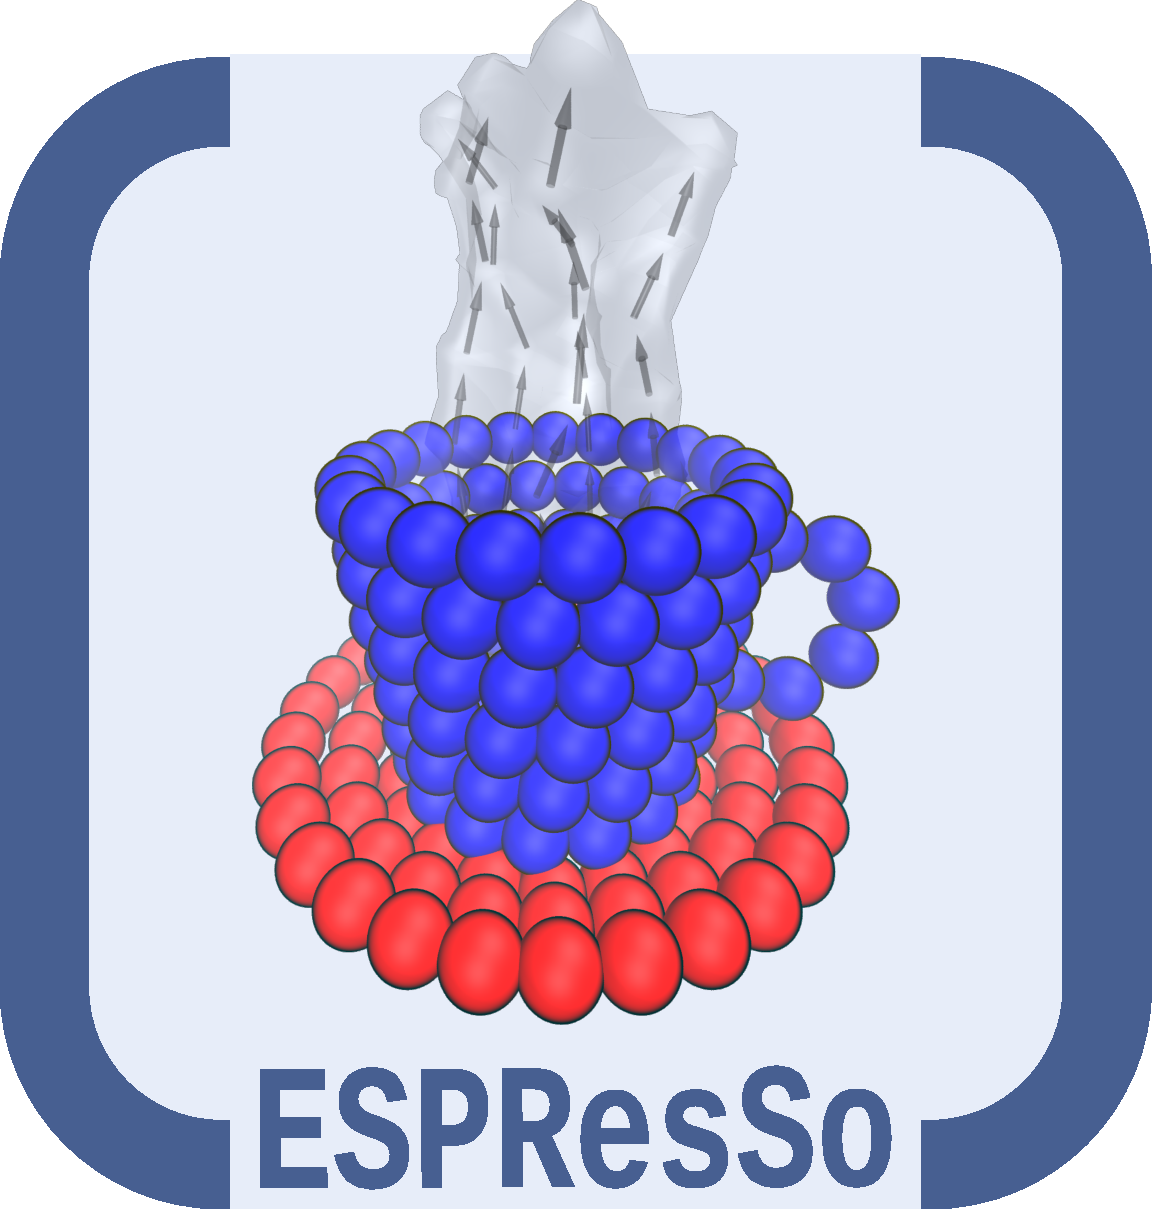
\includegraphics[width=5cm]{logo/logo.pdf}
    \end{center}
  }
}

% Copyright (C) 2010-2019 The ESPResSo project
% Copyright (C) 2002,2003,2004,2005,2006,2007,2008,2009,2010
%  Max-Planck-Institute for Polymer Research, Theory Group
%  
% This file is part of ESPResSo.
%   
% ESPResSo is free software: you can redistribute it and/or modify it
% under the terms of the GNU General Public License as published by the
% Free Software Foundation, either version 3 of the License, or (at your
% option) any later version.
%  
% ESPResSo is distributed in the hope that it will be useful, but
% WITHOUT ANY WARRANTY; without even the implied warranty of
% MERCHANTABILITY or FITNESS FOR A PARTICULAR PURPOSE.  See the GNU
% General Public License for more details.
%  
% You should have received a copy of the GNU General Public License
% along with this program.  If not, see <http://www.gnu.org/licenses/>.
%
\usepackage[draft]{varioref}    % defines \vref
\usepackage{hyperref}           % automatically creates links when
                                % using pdflatex, defines \url
\usepackage{ifpdf}              % defines \ifpdf
\usepackage{graphicx}           % handles graphics
\usepackage{color}              % use colors

\usepackage{amsmath}

\usepackage{verbatim}           % required for \verbatim and \endverbatim
\usepackage{fancyvrb}
\usepackage{calc}               % compute length
\usepackage{ifthen}             % provide ifthen
\usepackage{xspace}
\usepackage{units}
\usepackage[numbers]{natbib}

\usepackage{listings}

% For building the distribution docs, disable todo boxes.
%\usepackage[disable]{todonotes}
\usepackage{todonotes}

\newcommand{\es}{\mbox{\textsf{ESPResSo}}\xspace}
\newcommand{\ie}{\textit{i.e.}\xspace}
\newcommand{\eg}{\textit{e.g.}\xspace}
\newcommand{\etal}{\textit{et al.}\xspace}

\newcommand{\codebox}[1]%
{\texttt{#1}}

\DefineVerbatimEnvironment{code}{Verbatim}%
{commandchars=\\\{\}}
\makeatletter
\newenvironment{tclcode}
{%
  \addtolength{\linewidth}{-2em}% set the line length
  \@minipagetrue%%%DPC%%%
  \@tempswatrue%%%DPC%%%
  \hsize=\linewidth%
  \setbox0=\vbox\bgroup\verbatim
}{\endverbatim
  \unskip\setbox0=\lastbox%%%DPC%%%
  \egroup
  \par%
  \noindent\hspace{1em}%
  \codebox{\box0}%
  \par\noindent%
}
\makeatother

% \newcommand{\todo}[1]{
%   \marginpar{%
%     \setlength{\fboxrule}{1pt}
%     \fcolorbox{red}{yellow}{%
%       \parbox{\marginparwidth-2\fboxrule-2\fboxsep}{%
%         \bf\raggedright\scriptsize #1%
%       }%
%     }%
%   }%
% }

\makeatletter
\renewcommand{\minisec}[1]{\@afterindentfalse \vskip 1.5ex
  {\parindent \z@
    \raggedsection\normalfont\sffamily\itshape\nobreak#1\par\nobreak}%
  \@afterheading}
\makeatother

\newcommand{\esptitlehead}{
  \titlehead{
    \begin{center}
      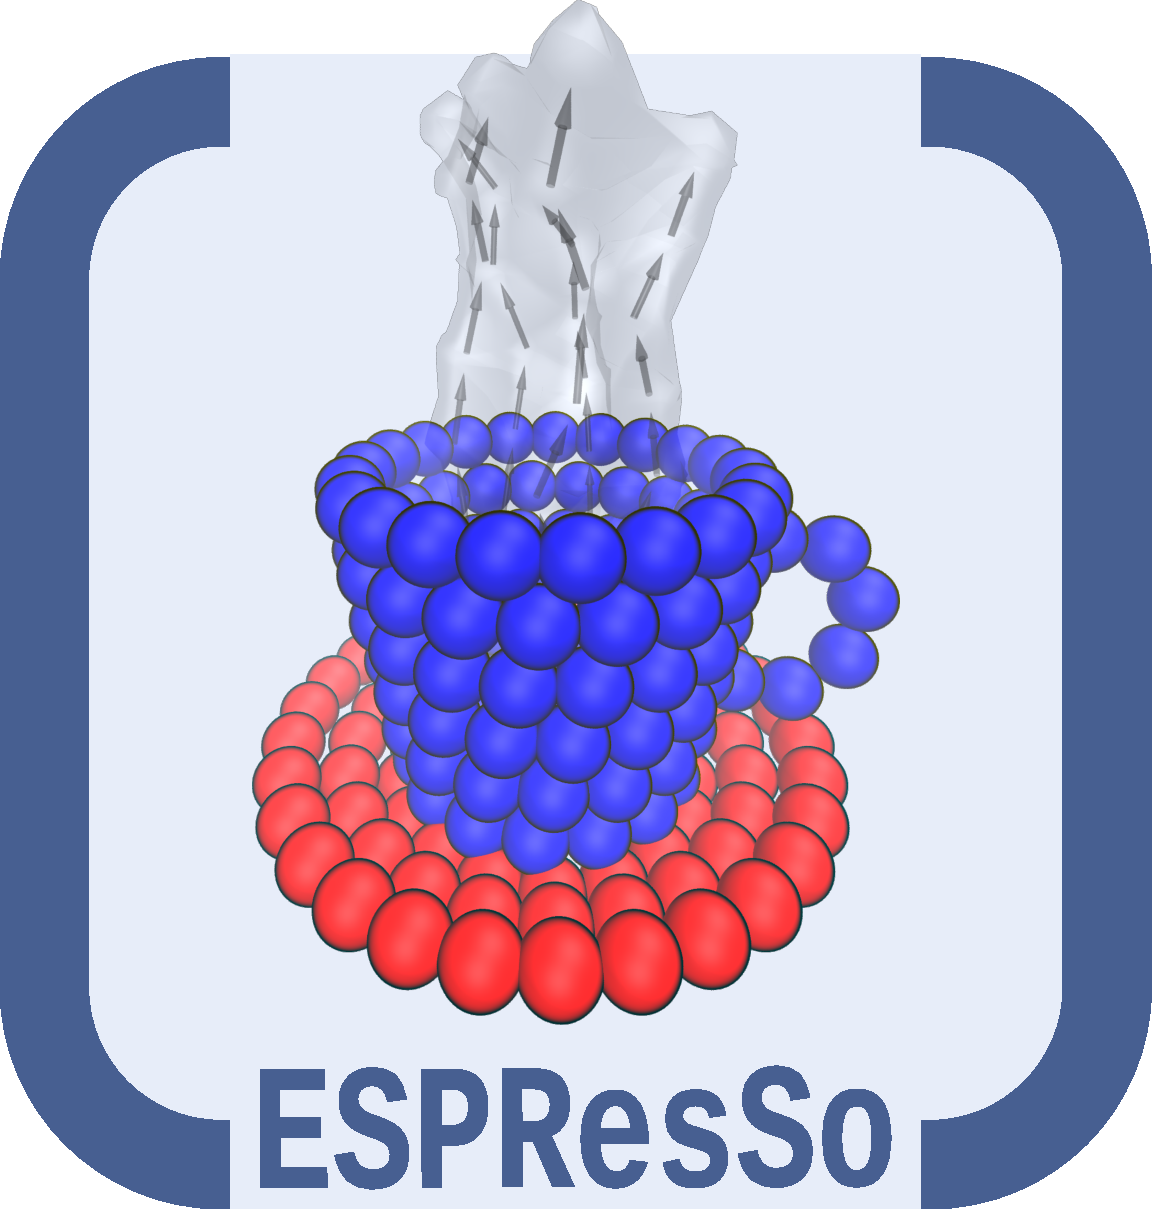
\includegraphics[width=5cm]{logo/logo.pdf}
    \end{center}
  }
}

\input{misc/common}







\begin{document}
\title{Tutorial 10: Reaction Ensemble and Constant pH ensemble}
\author{Andrea Tagliabue, Jonas Landsgesell}

\maketitle
\tableofcontents

\section{Introduction}

This tutorial introduces the basic features for simulating titratable systems via two different methods, the Constant pH method and the Reaction Ensemble method, pointing out differences and similarities between these two approaches and explaining the reasons to prefer the latter in some particular cases.
The first part (example one) of this tutorial will consider a homogeneous aqueous solution of a titratable acidic species HA that can dissociate as follows
\begin{equation}\label{disso}
\ce{HA <--> A- + H+}\text{,}
\end{equation}
while the second part (example two) will consider a polyelectrolyte chain formed by a series of titratable monomers bonded together.

\noindent Both constant pH and Reaction Ensemble methods are implemented via a Monte Carlo algorithm with the classical Metropolis-Hastings acceptation rule. Here we compare both methods based on the paper published by Landsgesell et. al\cite{landsgesell2017simulation}.

\section{Theoretical Background}

In this tutorial we deal with chemical reactions of the following kind:
\begin{equation}\label{disso}
\ce{HA <--> A- + H+}\text{.}
\end{equation}
If $N_0 = N_{\text{HA}} + N_{\text{A}^-}$ is the number of titratable groups in solution, a degree of dissociation $\alpha$ can be defined:
\begin{equation}\label{alpha}
\alpha = \frac{N_{\text{A}^-}}{N_0}.
\end{equation}
Another observable is the degree of association which is given by:
\begin{equation*}
\overline{n}=\frac{N_\text{HA}}{N_0}=1-\alpha.
\end{equation*}
The equilibrium concentration of each species is defined by the equilibrium reaction constant
\begin{equation}
K =\exp(\beta \sum_i \nu_i(\mu_i-\mu_i^0) )= \frac{a(\text{A}^-)a(\text{H}^+)}{a(\text{HA})};
\end{equation}
for each species $i$ $a(i)=e^{\beta (\mu_i-\mu_i^0)} = (c_i/c_{i}^{0})\gamma_i$ denotes the relative activity, $\mu_i$ is the chemical potential, $\mu_i^0$ is the chemical potential under some standard reference conditions, $\nu_i$ is the stoichiometric coefficient, $\gamma_i$ is the activity coefficient, $c_{i}$ and $c_{i}^{0}$ are the concentration of the species $i$ and its standard concentration, respectively. In the case of non-interacting particles (ideal gas) or very dilute solutions ($\gamma_i \approx 1$) activities are equal to $c_i/c_{i}^{0}$. In chemical equilibrium, which is defined by $\Delta G=\sum_i \nu_i \mu_i=0$, we obtain that $K=\exp(\beta \Delta (G-G^0))=\exp(-\beta \sum_i \nu_i \mu_i^0)$.
Therefore we have (in the case of no interactions):
\begin{equation}
\label{(eq5)}
\exp( \beta [ (\mu_{\text{H} ^+}- \mu_{\text{H}^+}^0)  +  (\mu_{\text{A}^-} - \mu_{\text{A}^-}^0) - (\mu_\text{HA} - \mu_\text{HA}^0) ])=
\prod_i \left( \frac{c_i}{c_i^0} \gamma_i \right)^{\nu_i} = \text{const} \text{.} 
\end{equation}
Equivalently, for reaction (\ref{disso}) and in case of a dilute solutions ($\gamma_i \approx 1$), equation (\ref{(eq5)}) can be approximated as follows:
\begin{equation}
K_{\text{c}} = \frac{c_{\text{H}}c_{\text{A}}}{c_{\text{HA}}}=\text{const},
\end{equation}
where $K_{\text{c}}$ carries the dimension 1/volume.


\subsection{Constant pH method}

In the constant pH method, the acceptance probability for a reaction is

\begin{equation} 
P_{\text{acc}} = \text{min}\left\lbrace  1, e^{\beta \Delta E_\text{pot} \pm \ln{10} (\text{pH - pK}_\text{a})}\right\rbrace \text{,}
\end{equation}
and the acceptance probability of a reaction is $P_\text{acc}=\frac{N_\text{HA}}{N0}$ for a dissociation and $P_\text{acc}=\frac{N_\text{A}}{N0}$ for an association reaction \cite{landsgesell2017simulation}. Here $\Delta E_\text{pot}$ is the potential energy change due to the reaction, while $\text{pH - p}K_\text{a}$ is an input parameter composed by two terms, pH and -p$K_\text{a}$, that represent, respectively, the concentration of \ce{H+} ions in the solution and the logarithm in base 10 of the thermodynamic dissociation constant for HA when the system is approximated as a dilute solution ($\gamma_i \approx 1$):
\begin{equation} 
\text{pH} = -\log_{10} \frac{c_{\text{H}^+}}{c_{\text{H}^+}^0}\text{;}
\end{equation}
\begin{equation} 
K_\text{a} = \frac{(c_{\text{H}^+}/c_{\text{H}^+}^0)(c_{\text{A}^+-}/c_{\text{A}^+-}^0)}{(c_{\text{HA}}/c_{\text{HA}}^0)} \text{.}
\end{equation}
The chemical prefactor $\pm 1$ defines the direction of the reaction (+1 dissociation, -1 association).
When a dissociation move is attempted, the titratable molecule HA is charged and a counterion \ce{H+} is randomly placed into the simulation box, while when an association move is attempted, a \ce{A-} is neutralized and a random counterion \ce{H+} is removed from the cell.


\subsection{Reaction Ensemble method}
A chemical reaction involving ${n}$ species of type ${s_i}$ and with stoichiometric coefficients $\nu_i$ can be written as 
\begin{equation}
\sum_{i = 1}^n \nu_{i} s_i = 0\text{.}
\end{equation}
For such a general reaction, the acceptance probability in the Reaction Ensemble method is defined as
\begin{equation}\label{RE}
P_{\text{acc}} = \text{min} \left\lbrace 1, K_{c}^\xi V^{\bar{\nu}\xi} \prod_{i = 1}^{n} \left[ \frac{N_{i}^0!}{(N_{i}^{0} + \xi \nu_i)}  \right] e^{-\beta \Delta E_\text{pot}}  \right\rbrace\text{.}
\end{equation}
Here $K_c$ is the ideal reacting gas quantity introduced above, $V$ the volume, $\bar{\nu}$ the total change in the number of particles, $N_0^i$ the number of particles prior to the reaction and $\xi$ is the extent of the reaction, which could assume value +1 (forward reaction) or -1 (backward reaction). Each reaction is proposed with uniform probability. 

\noindent For reaction (\ref{disso}) eq. (\ref{RE}) can be simplified: 
\begin{equation}
P_{\text{acc}} = \text{min} \left\lbrace 1, (  K_c \frac{N_{\text{HA}}}{N_\text{A} - N_{\text{H}+}/V)} e^{-\beta \Delta E_\text{pot}}  \right\rbrace\text{.}
\end{equation}
Notice that in this case you can also define $K_\text{a} = K_c/c_0$ .

The main difference in the two methods consists in the fact that in the Reaction Ensemble the system pH is determined via the actual proton concentration in the simulation box, while in Constant pH method it represents an input parameter which remains constant during all the simulation.


\section{Example one: homogeneous aqueous solution of acidic species}

Compile Espresso with the following features in your
\texttt{myconfig.hpp} to be set throughout the whole tutorial:

\begin{verbatim}
# define LENNARD_JONES
# define ELECTROSTATICS
\end{verbatim}

\subsection{System Setup}

We start by defining some important input parameters and setting the particles randomly inside the box:
\begin{verbatim}
import espressomd
from espressomd import reaction_ensemble

box_l = 15        #side length of our cubic simul box
system = espressomd.System(box_l=[box_l]*3)

system.set_random_state_PRNG()
np.random.seed(seed=system.seed)


# Particle setup
#############################################################
# type 0 = HA
# type 1 = A-
# type 2 = H+

N0 = 50             #number of titratable particles
K_diss = 8.3**(-4)  #dissociation costant 
 
# titratable particles (HA)
for i in range(N0):
    system.part.add(id=i, pos=np.random.random(3) * system.box_l, type=1)
# counterions (H+)   
for i in range(N0, 2 * N0):
    system.part.add(id=i, pos=np.random.random(3) * system.box_l, type=2)
\end{verbatim}

For each negatively charged \ce{A-} particle (type = 1) we put in the simulation box the respective counterion \ce{H+} (type = 2) in order to maintain the electroneutrality of the system.
Notice that the implementation in Espresso requires that the dimension of the equilibrium constant is consistent with its internal unit of volume; rules for a correct conversion of $K_a$ (experimental) to $K_c$ (in internal units) are explained in the user guide: \url{http://espressomd.org/html/doc/advanced_methods.html}. The next step is to define the reaction system and seed the pseudo random number generator which is used for the Monte Carlo steps:

\begin{verbatim}
mode="reaction_ensemble"
#mode="constant_pH_ensemble"

RE=None
mode=="reaction_ensemble"
if(mode=="reaction_ensemble"):
    RE = reaction_ensemble.ReactionEnsemble(temperature=1, exclusion_radius=1, seed=42)
elif(mode=="constant_pH_ensemble"):
    RE = reaction_ensemble.ConstantpHEnsemble(temperature=1, exclusion_radius=1, seed=42)
    RE.constant_pH=7
    
RE.add_reaction(gamma=K_diss, reactant_types=[0], reactant_coefficients=[1], 
product_types=[1, 2], product_coefficients=[1, 1], default_charges=
{0: 0, 1: -1, 2: +1})

system.setup_type_map([0, 1, 2])
\end{verbatim}
You can switch from one method to the other simply by changing the \texttt{mode} parameter from \texttt{"reaction\_ensemble"} to \texttt{"constant\_pH\_ensemble"}. Now the system is ready to be simulated.

\begin{verbatim}
Nreac = 10**4 #number of association/dissociation attempt to be performed
for i in range(Nreac):
    RE.reaction()
\end{verbatim}
Notice that, at this level, we're not taking into account electrostatic interactions between charged species. Therefore, if you compare the input equilibrium constant $K_c$ and the effective one which can be calculated at the end of a simulation run $K_c^{\text{(eff)}} = \frac{\langle c_{\text{A}^-} \rangle \langle c_{\text{H}^+} \rangle }{\langle c_\text{HA} \rangle}$ you will obtain $K_c \simeq K_c^\text{(eff)}$. This is not true when e.g. electrostatic interactions are enabled due to the fact the latter introduces an excess chemical potential.


\subsection{Dissociation degree versus concentration}

Performing several simulations with constant $N_0$ but varying the dimension of the simulation box it is possible to obtain the dissociation degree $\alpha$ (eq. \ref{alpha}) as a function of the concentration of titratable units. Results are shown in figure \ref{alpha_vs_C}.
\begin{figure}[tb]
	\centering
 	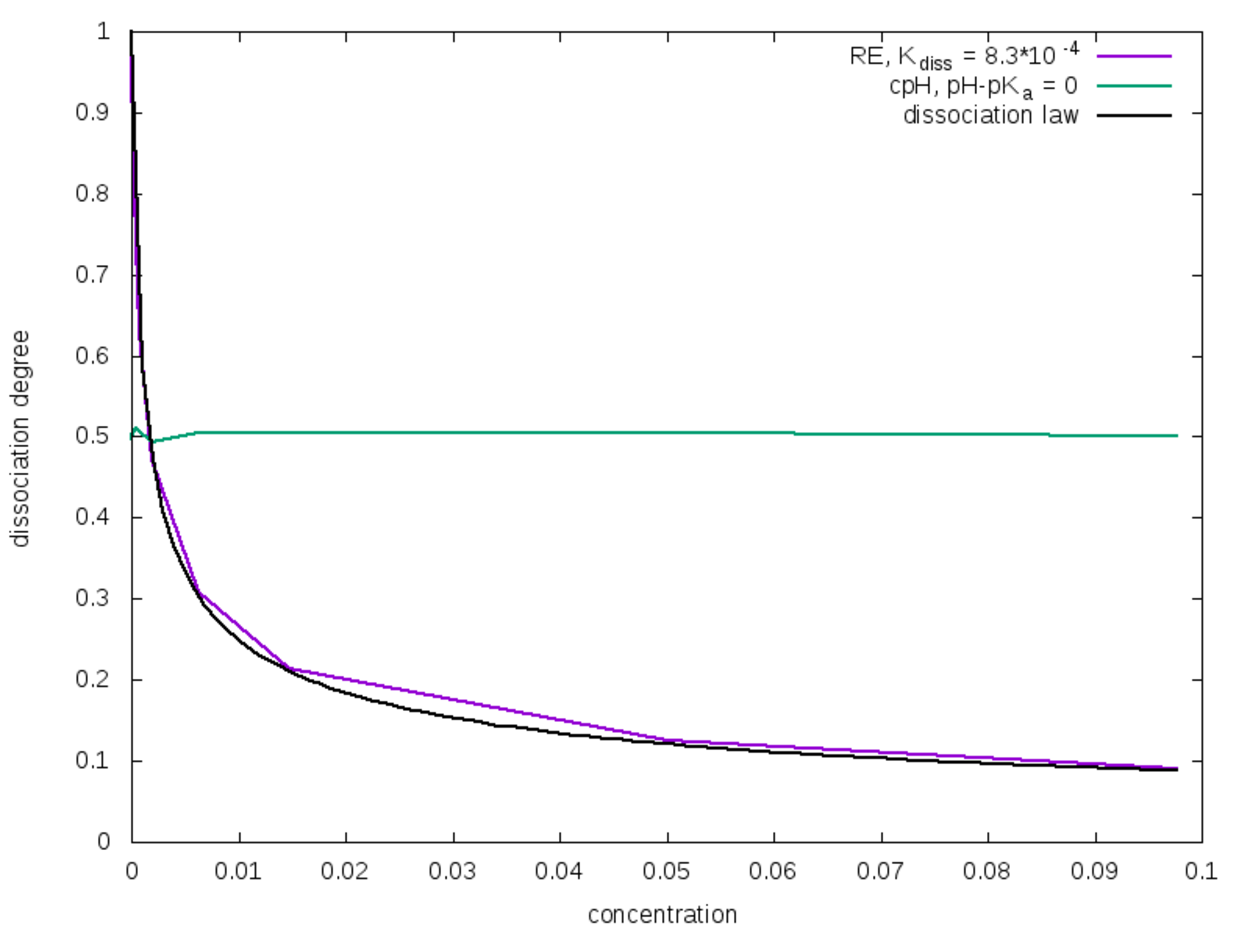
\includegraphics[scale=0.6]{figures/alpha_vs_C.pdf}
 	\caption{Dissociation degree $\alpha$ as function of the concentration of titratable groups. Yellow squares: Constant pH method; light blue triangles: Reaction Ensemble method; blue solid line: ideal behavior.}
 	\label{alpha_vs_C}
\end{figure}
As you can see, only the curve obtained with the Reaction Ensemble method fits the ideal behavior described by the dilution law
\begin{equation}
K_{a} = \frac{\alpha^2}{1 - \alpha}c_\text{titr}\text{,}
\end{equation}
where $c_\text{titr}$ is the concentration of titratable units in the solution, and this is due to the fact that the acceptance rule in Constant pH method does not depend on the volume of the system. As $\alpha$ differs, so will the number of counterions in the cell. This could have a strong impact on screening effects when electrostatic interactions are taken into account. Moreover, in the Constant pH method the real chemical nature of counterions is unknown. In fact, when a HA molecule dissociates at high pH value, the generated \ce{H+} would react instantaneously with an \ce{OH-} ions, so the positively charged ions that remains in solution must represent a different species (e.g. a \ce{Na+} cation).




\section{Example two: linear weak polyelectrolytes}
Weak polyelectrolytes are a family of responsive materials whose application spans the range from flocculation-induced water purification to tissue targeted drug delivery of expensive or cytotoxic medicines. Their properties, however, depend on their specific chemical environment, with details such as pH, salt concentration and valency, and their topology markedly modifying the chemical behavior of their ionizing groups.
Here we're going to study the titration curves of a linear weak polyelectrolyte composed by 50 titratable units with both Reaction Ensemble and Constant pH methods. In this case, we'll enable electrostatic interactions between charged species in order to correctly describe their properties.

\subsection{System setup}

First of all, we start to define some important variables and create a dictionary containing the type and the charge for all the species in solution (this could be very useful when you have to handle with a lot of different species in your simulations):
\begin{verbatim}
# system parameters
box_l = 56.134
l_bjerrum = 2.0 
temperature = 1.0

system = espressomd.System(box_l=[box_l]*3)

# particle setup
N_P = 1       #number of chains
MPC = 50      #monomers per chain
N0 = N_P*MPC  #total number of monomers
nNaOH = 0     #number of initial Na+OH-
nHCl = 0      #number of initial H+Cl- (additional H+'s)

type_HA = 0   # type 0 = HA
type_A  = 1   # type 1 = A-
type_H  = 2   # type 2 = H+
type_OH = 3   # type 3 = OH-
type_Na = 4   # type 4 = Na+
type_Cl = 5   # type 5 = Cl-

charges={}
charges[type_HA] =  0    
charges[type_A]  = -1     
charges[type_H]  =  1
charges[type_OH] = -1
charges[type_Na] =  1
charges[type_Cl] = -1 
\end{verbatim}
Here, we've defined the type and the charge of polymer titratable units (\ce{HA <--> A-}), counterions \ce{H+}, and additional ionic species (\ce{Na+OH-} and \ce{H+Cl-}) that can be inserted inside the simulation box. Now we have to set up all these particles and to define all the interactions.
\begin{verbatim}
# bonding interactions
bond_l = 1.2       #bond length
kbond = 100        #force constant for harmonic bond
harmonic_bond = interactions.HarmonicBond(k=kbond, r_0=bond_l)
system.bonded_inter.add(harmonic_bond)

# non-bonding interactions parameters
lj_eps   = 1.0
lj_sig   = 1.0
lj_cut   = 1.12246
lj_shift = 0.0

# setting up the polymer
polymer.create_polymer(N_P = N_P, bond_length = bond_l, MPC=MPC, start_id=0,
 bond=harmonic_bond, type_poly_neutral=type_HA, type_poly_charged=type_A, mode=0,
  val_poly=charges[type_A])
  
# setting up counterions
for i in range(N0):
    system.part.add(pos=np.random.random(3) * system.box_l, type=type_H, 
    q=charges[type_H])

# setting up other background ions
# - Na+ and OH-
for i in range(nNaOH):
    system.part.add(pos=np.random.random(3) * system.box_l, type=type_OH,
    q=charges[type_OH])
for i in range(nNaOH):
    system.part.add(pos=np.random.random(3) * system.box_l, type=type_Na,
    q=charges[type_Na])
# - (additional) H+ and Cl-
for i in range(nHCl):
    system.part.add(pos=np.random.random(3) * system.box_l, type=type_H, 
    q=charges[type_H])
for i in range(nHCl):
    system.part.add(pos=np.random.random(3) * system.box_l, type=type_Cl, 
    q=charges[type_Cl])
\end{verbatim}
As already explained, we need to enable electrostatic interactions to correctly simulate the physics of this type of system.
\begin{verbatim}
# setting up electrostatics
from espressomd import electrostatics
p3m = electrostatics.P3M(prefactor = l_bjerrum*temperature, accuracy=1e-3) 
system.actors.add(p3m)
\end{verbatim}
To titrate a weak polyelectrolytic chain, which is composed by $N_0$ titratable units with a certain $\text{p}K_a$, in the Reaction Ensemble, we need to modulate the pH of the environment. To do this, we have to add additional \ce{H+} ions, increasing the pH, or \ce{OH-} ions, to decrease it. We have also to introduce the respective counterions (\ce{Cl-} or \ce{Na+}) to preserve the electroneutrality of the system. Finally, we have to take into account also the autoprotolysis of water (\ce{H2O <--> H+ + OH-}) beside the main dissociation reaction.

\begin{verbatim}
K_diss = 1.0*0.002694         #eq constant HA <--> A- + H+
# 0.00269 is the conversion constant from mol/L to internal units
# when sigma is 3.55 angstrom

K_w = 10.0**(-14)*0.02694**2  #eq constant for autoprotolysis
# notice that here we converted the value from (mol/L)^2 to 
# internal units 

#HA <--> A- + H+
RE.add_reaction(gamma=K_diss, reactant_types=[type_HA],
    reactant_coefficients=[1],    product_types=[type_A, type_H], 
    product_coefficients=[1,1], default_charges={type_HA: charges[type_HA], 
    type_A: charges[type_A], type_H: charges[type_H]})

#H2O autoprotolysis 
RE.add_reaction(gamma=(1/K_w), reactant_types=[type_H, type_OH], 
reactant_coefficients=[1,1], product_types=[],    product_coefficients=[],    
default_charges={type_H: charges[type_H], type_OH: charges[type_OH]})
\end{verbatim}
Please notice that the order in which the species are written in reactants and products lists is very important because, when a reaction is performed, the first species in the reactants list is replaced by the first species in the product lists, the second reactant species is replaced by the second product species, and so on. Moreover, if the reactant list has more species than the products list, reactant molecules in excess are deleted from the system, while if the products list has more species than the reactants list, product molecules in excess are created and randomly placed inside the simulation box. For example, reversing the order of products in our reaction (i.e. from  \verb|product_types=[type_H, type_A]| to \verb|product_types=[type_A, type_H]|), a neutral monomer would be positively charged and a negative monovalent counterion would be randomly placed inside the cell. 

Due to the fact that, at a certain pH, the ionization degree of a weak polyelectrolytes depends on its spatial conformation, in order to obtain  correctly averaged values we have also to couple the reaction algorithm with MD simulations. 
\begin{verbatim}
# Integration parameters
system.time_step = 0.01
system.cell_system.skin = 10. #only for tutorial purposes 
system.cell_system.max_num_cells = 2744
system.thermostat.set_langevin(kT=temperature, gamma=1.0, seed=42)
\end{verbatim}
Finally, we are ready to run the simulation!
\begin{verbatim}
for i in range(12000):
    RE.reaction(50)
    system.integrator.run(500) 
    print(i,") HA", system.number_of_particles(type=type_HA), "A-",
     system.number_of_particles(type=type_A), "H+",
      system.number_of_particles(type=type_H), 'OH-',
       system.number_of_particles(type=type_OH), 'Cl-',
        system.number_of_particles(type=type_Cl), 'NA+',
         system.number_of_particles(type=type_Na))
\end{verbatim}



\subsection{Titration curves}

\begin{figure}[h]
	\centering
	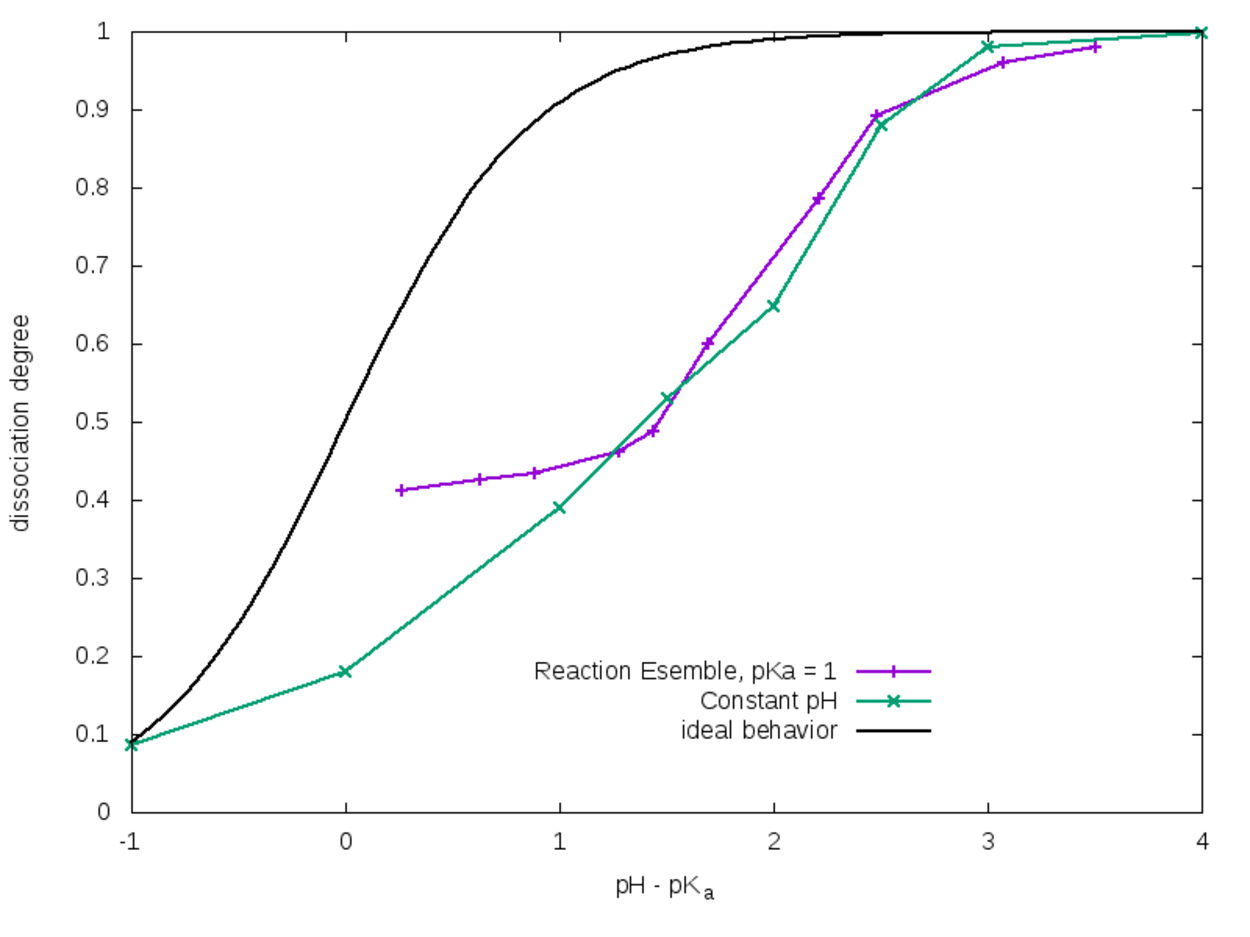
\includegraphics[scale=0.6]{figures/titration.pdf}
	\caption{Titration curves for a linear weak polyelectrolyte chain composed by $N_0=50$ titratable monomers. Yellow squares: Constant pH method; light blue triangles: Reaction Ensemble method; blue solid line: ideal behavior.}
	\label{titration}
\end{figure}
For a solution of weak acidic molecules with a certain $\text{p}K_\text{a}=-\log_{10}(K_c/c^0)$, the trend of $\alpha$ as function of pH is described by the Henderson-Hasselbalch equation:
\begin{equation}
\text{pH} = -\log_{10}(c_{\text{H}^+})/c^0).
\end{equation}
However, when titratable units are bonded together in a polyelectrolyte chain their effective $\text{p}K_\text{a}^\text{(eff)}$ differs from the ideal one ($\text{p}K_\text{a}$); this can be explained by the fact that the charge carried by a dissociated monomer tends to partially inhibit the dissociation of its neighbors, and this results into a lower total degree of dissociation with respect to the non-bonded acidic units case. Anyway, this effect can be partially compensated by the presence of counterions, which are able to  screen repulsive interactions between dissociated monomers. As you can observe in figure \ref{titration}, Constant pH and Reaction Ensemble method results are very similar at high pH values, but they show very pronounced differences at low pH values. More in details, $\text{p}K_\text{a}^\text{(eff)}$ tends to the ideal one when the concentration of \ce{H+} is high. This depends on the fact that with Reaction Ensemble method we have to inject a strong acid (\ce{H+}\ce{Cl-}) in order to titrate the polymer, and this results in a more salty solution with a strong screening power. This behavior would be reversed in case of a weak poly-base, with superimposable curves at low pH values and the Reaction Ensemble one approaching the ideal one when the amount of \ce{OH-} ions becomes relevant.
 

\section{Charge distribution along the chain}

\begin{figure}[h]
	\centering
	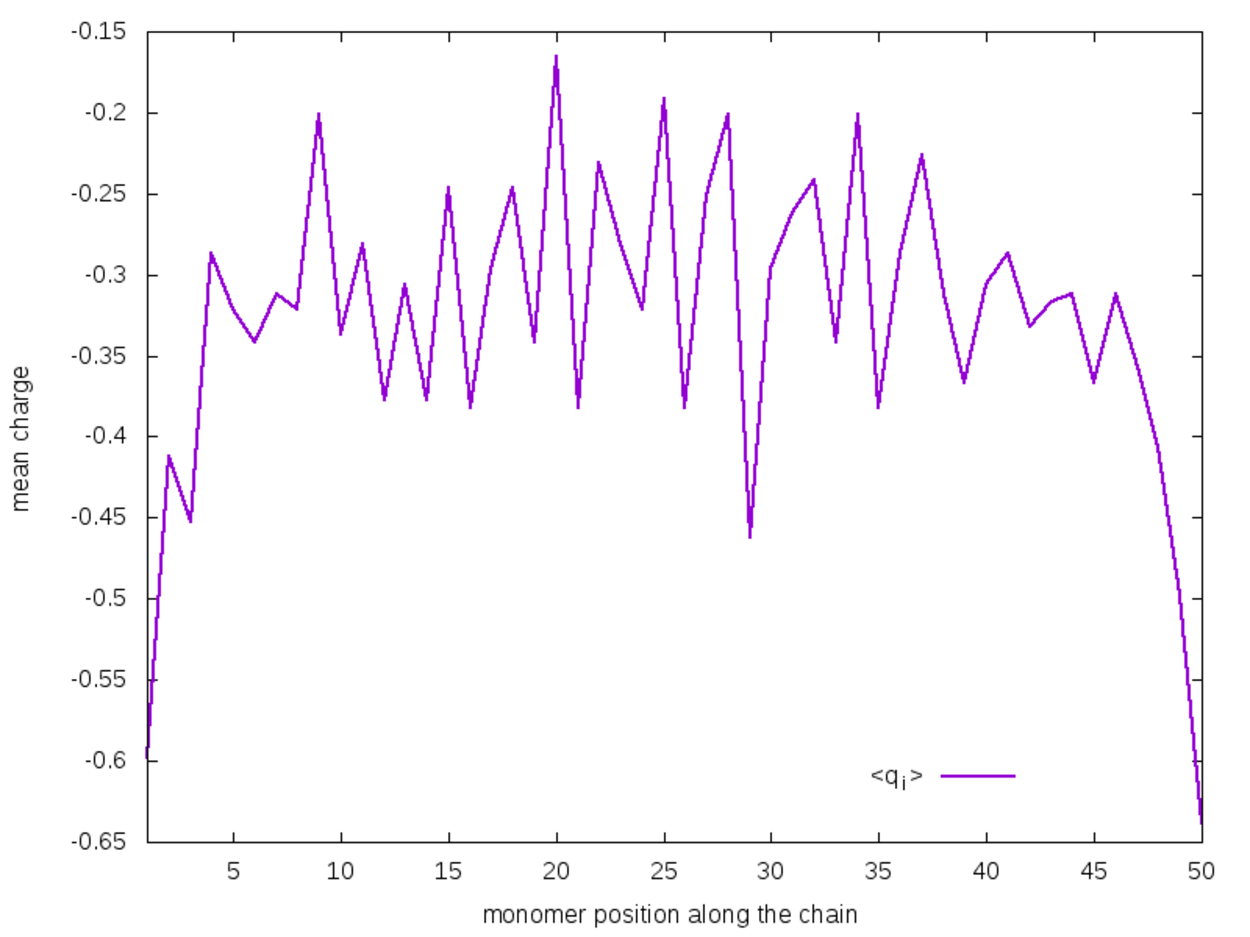
\includegraphics[scale=0.6]{figures/qdistrib.pdf}
	\caption{Mean charges of monomers as function of their position along the chain (calculated via Reaction Ensemble method) at $\alpha \simeq 0.4$ Notice that the curve is noisy because of the short duration of the simulation. Make sure to perform longer simulations to achieve a better convergence.}
	\label{qdistrib}
\end{figure}
Figure \ref{qdistrib} shows the mean charge assumed by each monomer during the simulation as a function of its position along the chain. As you can observe, monomers lying at the extremities tend to be more charged than those lying in the innermost regions. This could be easily explained thinking that the ends of the chain can better arrange in space in order to minimize repulsive interactions between charges. This results do not depend on the method, i.e. the shape of the curve at a certain dissociation degree would be te same also with the Constant pH; however, as previously discussed, at a certain value $\text{pH - p}K_\text{a}$, the total dissociation degree is method-dependent, so the Constant pH curve would be shifted to lower mean charge values for a weak poly-acid at high pH values.

\bibliographystyle{unsrt}
\bibliography{references}

\end{document}
